\section{Experiments \& Results}
\label{sec:experiments}
\subsection{Mục tiêu và tập thực nghiệm}
Thực nghiệm đánh giá năm mã hóa SAT và bốn mô hình/bộ giải đối sánh theo yêu cầu đề bài \citep{assignment}. Các tiêu chí gồm mức độ hoàn tất, thời gian sinh/nạp/giải, thời gian toàn lượt, kích thước biểu diễn và RSS. Tất cả số đo trong phần này lấy từ đợt \texttt{20261015T101136Z\_afe2720f}; không ghép thời gian của đợt một tầng hoặc của tài liệu tham khảo.

Tập kích thước là
\begin{equation}
\begin{split}
\mathcal N=\{&4,8,9,16,25,27,36,49,64,81,100,125,\\
&216,343,512,729,1000,1331\}.
\end{split}
\end{equation}
Đây là hợp các bình phương và lập phương của các số nguyên từ 2 đến 11, loại trùng và sắp tăng; cách chọn cũng được dùng trong tài liệu N-Queens tham khảo \citep{bach2024}. Mỗi đầu vào là một bàn cờ trống chuẩn, không có hậu cố định hoặc ô cấm. Mục tiêu là tìm một nghiệm, không liệt kê tất cả nghiệm hoặc tối ưu một hàm mục tiêu khác.

Mỗi cặp kích thước--cấu hình được chạy ba lần, tổng $18\times9\times3=486$ lượt. Năm tên SAT trong CSV vẫn là Binomial, Binary, Sequential, Commander và Product; hai tên cuối chỉ các cài đặt đệ quy của Phần~\ref{sec:methodology}. Bộ thực nghiệm lớn không chứa các ca UNSAT $N=2,3$, nên tỷ lệ thành công ở đây đo việc tìm nghiệm trong ngân sách, không đánh giá hiệu năng chứng minh UNSAT.

\subsection{Môi trường và tham số}
\begin{table}[pos=H]\centering\small
\caption{Môi trường và cấu hình được ghi trong manifest của đợt mới.}
\label{tab:environment}
\begin{tabular}{@{}p{.27\linewidth}p{.66\linewidth}@{}}\toprule
Thuộc tính & Giá trị\\\midrule
CPU & Intel64 Family 6 Model 186 Stepping 2, GenuineIntel; 8 nhân vật lý, 12 CPU lôgic.\\
RAM / OS & 16034.38 MiB RAM; Windows 11, build 10.0.26200.\\
Python & 3.14.4.\\
SAT & Glucose3 qua python-sat 1.9.dev15.\\
CP-SAT & OR-Tools 9.15.6755.\\
CPLEX MIP & Gói cplex 22.2.0.0.\\
CPLEX CP & Gói docplex 2.32.264; phiên bản executable CP Optimizer chưa được ghi.\\
Gurobi / giám sát & gurobipy 13.0.3; psutil 7.2.2.\\
Ngân sách mỗi lượt & 100 giây toàn lượt; ngưỡng RSS quan sát 6144 MiB.\\
Giới hạn clause & \texttt{max\_clauses=0}: không bỏ qua theo kích thước CNF.\\
Lặp / luồng & Ba lần lặp; một luồng/worker theo cấu hình.\\
Seed & Native seed 0; order seed 2026; SAT không áp dụng seed riêng.\\
ALO / lô / lấy mẫu & ALO cột bật; tối đa 8192 clause/lô; khoảng lấy mẫu cấu hình 20 ms.\\
\bottomrule\end{tabular}
\end{table}
Bảng~\ref{tab:environment} sử dụng thông tin của manifest thay cho suy đoán từ máy tham khảo. Tên thương mại CPU, chế độ nguồn điện và phiên bản executable CP Optimizer chưa có trong dữ liệu. Phiên bản \texttt{docplex} là phiên bản giao diện Python, không thay thế phiên bản engine CP Optimizer. Những giới hạn này được giữ rõ trong đánh giá khả năng tái lập.

Các lượt được xáo thứ tự theo seed cố định để tránh luôn chạy một phương pháp trước mọi phương pháp khác. Ba lần lặp cùng cấu hình không phải ba seed SAT độc lập. Cấu hình một luồng của backend cũng không có nghĩa toàn hệ điều hành chỉ sử dụng một luồng, vì còn tiến trình cha và bộ giám sát.

\subsection{Định nghĩa phép đo và cách tổng hợp}
\subsubsection{Thời gian}
Với SAT, \texttt{build\_s} đo thời gian sinh các lô CNF, \texttt{load\_s} đo thời gian nạp chúng và \texttt{solve\_s} đo thời gian quanh lời gọi tìm nghiệm. Với CP/MIP, build đo xây mô hình; solve đo lời gọi adapter, có thể bao gồm xuất mô hình, presolve và giao tiếp với engine. Do đó native solve không được hiểu là chỉ thời gian tìm kiếm bên trong bộ giải.

Đặt $r$ là một lần lặp. Thời gian xử lý mô hình và giải được tính trước cho từng lượt:
\begin{equation}
T_{\mathrm{work},r}=\begin{cases}
T_{\mathrm{build},r}+T_{\mathrm{load},r}+T_{\mathrm{solve},r},&\text{SAT},\\
T_{\mathrm{build},r}+T_{\mathrm{solve},r},&\text{CP/MIP}.
\end{cases}
\end{equation}
Sau đó mới tính $\widetilde T_{\mathrm{work}}=\operatorname{median}(T_{\mathrm{work},1},T_{\mathrm{work},2},T_{\mathrm{work},3})$. Không cộng các trung vị build, load, solve để thay cho trung vị tổng.

\texttt{total\_s} là thời gian từ lúc khởi tạo worker đến khi nhận kết quả đã kiểm tra; theo manifest, thời gian ghi log và dọn dẹp sau đó không nằm trong total. Total còn chứa khởi động tiến trình, thiết lập thư viện, giải mã và phối hợp giữa các tiến trình. Ngưỡng 100 giây áp dụng cho toàn lượt, nên một công thức có thể bị dừng trong giai đoạn sinh/nạp trước khi solver bắt đầu tìm nghiệm. Các giá trị kết thúc hơi lớn hơn 100 giây phản ánh độ trễ giám sát và nhận kết quả, không được làm tròn ngược thành thời gian giải thành công 100 giây.

\subsubsection{Bộ nhớ và kích thước biểu diễn}
\texttt{peak\_rss\_mib} là giá trị lớn nhất quan sát được của tổng RSS worker và các tiến trình con. Nó bao gồm Python, thư viện, mô hình và bộ giải. Phép lấy mẫu 20 ms có thể bỏ sót đỉnh ngắn; trang chia sẻ có thể bị cộng lặp. Ngưỡng RSS của bộ giám sát không phải giới hạn cấp phát cứng do hệ điều hành bảo đảm.

Số biến/clause/literal SAT là kích thước CNF đầy đủ theo công thức, trước tiền xử lý và không gồm clause học. Các giá trị không thay đổi chỉ vì lượt chạy timeout. Hai cột clause đã sinh/nạp ghi tiến độ thực tế đã nhận. Với CP/MIP, số biến và ràng buộc là kích thước tại giao diện mô hình; một AllDifferent không tương đương một clause CNF.

\subsubsection{Trạng thái và lượt chưa hoàn tất}
\begin{table}[pos=H]\centering\small
\caption{Quy ước của các bảng thời gian trong báo cáo.}
\begin{tabular}{@{}lp{.73\linewidth}@{}}\toprule
Ký hiệu & Ý nghĩa\\\midrule
Giá trị số & Trung vị của ba lượt SAT có nghiệm hợp lệ.\\
TO & Cả ba lượt TIMEOUT.\\
2TO+1U & Hai lượt TIMEOUT và một lượt UNKNOWN.\\
1S+2TO & Một lượt SAT và hai lượt TIMEOUT.\\
-- & Không áp dụng hoặc chưa có số đo pha hoàn tất, theo chú thích bảng.\\
\bottomrule\end{tabular}
\end{table}
SAT trong các bản ghi native cũng chỉ việc tìm được nghiệm khả thi, không có nghĩa backend đó nhận đầu vào CNF. UNKNOWN là trạng thái dừng chưa xác định được SAT/UNSAT. Hai UNKNOWN thuộc CP-SAT: $N=343$ lượt 3, total 99.8114 giây; $N=729$ lượt 1, total 100.0006 giây. Cả hai có lý do \texttt{NATIVE\_STOP}; báo cáo không đổi chúng thành TIMEOUT hoặc UNSAT.

Khi một nhóm chưa hoàn tất đủ ba lượt, bảng chính giữ ký hiệu trạng thái, không lấy trung vị chỉ từ các lượt may mắn thành công. Các giá trị 0 chưa cập nhật trong trường solve của một lượt bị ngắt không phải thời gian giải bằng 0. Ngân sách 100 giây cũng không phải số đo thời gian cần để giải xong trường hợp đó. Thống kê Q1/Q3 và IQR chỉ mô tả ba lần lặp hoàn tất, không được dùng như khoảng tin cậy.

\subsection{Kiểm tra dữ liệu và mức độ hoàn tất}
CSV và JSONL chứa cùng 486 bản ghi, có 486 run ID khác nhau, cùng experiment ID, code hash và config hash. Tập lượt chạy khớp đầy đủ lưới cấu hình của manifest, không thiếu lần lặp. Tất cả 385 vector nghiệm được kiểm tra lại bằng~\eqref{eq:check} và hợp lệ. Có 128 nhóm hoàn tất 3/3, một nhóm hoàn tất 1/3 và 33 nhóm không có lượt thành công. Tổng trạng thái là 385 SAT, 99 TIMEOUT và 2 UNKNOWN; không có SKIPPED, MEM\_LIMIT hoặc ERROR.

Đối với SAT CNF, cả 270 dòng có số biến phụ, clause và literal khớp công thức của đúng biến thể. Trong 193 lượt SAT hoàn tất, số clause thực sinh và thực nạp đều bằng kích thước CNF đầy đủ. Đây là kiểm tra nhất quán số liệu cùng kiểm tra nghiệm, không thay thế việc kiểm thử generator và kiểm toán snapshot mã nguồn.
\begin{table}[pos=H]
\centering
\small
\caption{Mức độ hoàn tất của đợt thực nghiệm không giới hạn clause.}
\label{tab:coverage}
\setlength{\tabcolsep}{4pt}
\begin{tabular}{@{}lrrrrr@{}}
\toprule
Phương pháp & Đủ 3/3 & Có SAT & SAT & TO & UNK \\
\midrule
Binomial & 13/18 & 13/18 & 39 & 15 & 0 \\
Binary & 15/18 & 15/18 & 45 & 9 & 0 \\
Sequential & 12/18 & 12/18 & 36 & 18 & 0 \\
Commander & 13/18 & 13/18 & 39 & 15 & 0 \\
Product & 11/18 & 12/18 & 34 & 20 & 0 \\
CP-SAT & 13/18 & 13/18 & 39 & 13 & 2 \\
CPLEX CP & 18/18 & 18/18 & 54 & 0 & 0 \\
CPLEX MIP & 16/18 & 16/18 & 48 & 6 & 0 \\
Gurobi & 17/18 & 17/18 & 51 & 3 & 0 \\
\bottomrule
\end{tabular}
\par\smallskip\begin{minipage}{\linewidth}\footnotesize Hai cột tỷ lệ đếm kích thước; ba cột cuối đếm lượt. Mỗi phương pháp được thử đủ 54 lượt; không có SKIPPED, MEM\_LIMIT hoặc ERROR.\end{minipage}
\end{table}

\begin{figure}[pos=H]\centering
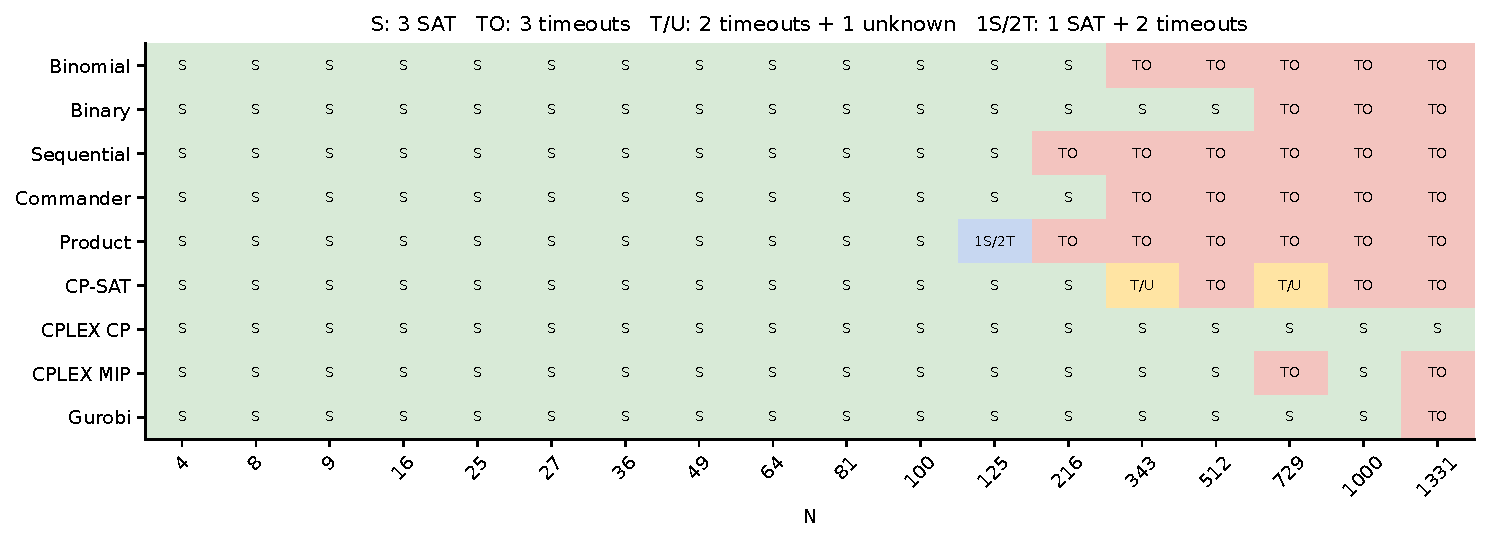
\includegraphics[width=\linewidth]{figures/status_matrix.pdf}
\caption{Trạng thái trên 18 kích thước. S: ba lượt SAT; TO: ba TIMEOUT; T/U: hai TIMEOUT và một UNKNOWN; 1S/2T: một SAT và hai TIMEOUT.}
\label{fig:status}
\end{figure}
CPLEX CP hoàn tất cả 18 kích thước; Gurobi hoàn tất 17; CPLEX MIP 16; Binary 15; Binomial, Commander và CP-SAT cùng 13; Sequential 12; Product hoàn tất đủ ba lượt ở 11 kích thước và có một lượt thành công thêm tại $N=125$. Tất cả cấu hình đều đã được thử ở mọi kích thước, nên không còn sự nhập nhằng giữa bỏ qua trước chạy và timeout trong đánh giá mức độ hoàn tất.

\begin{figure}[pos=H]\centering
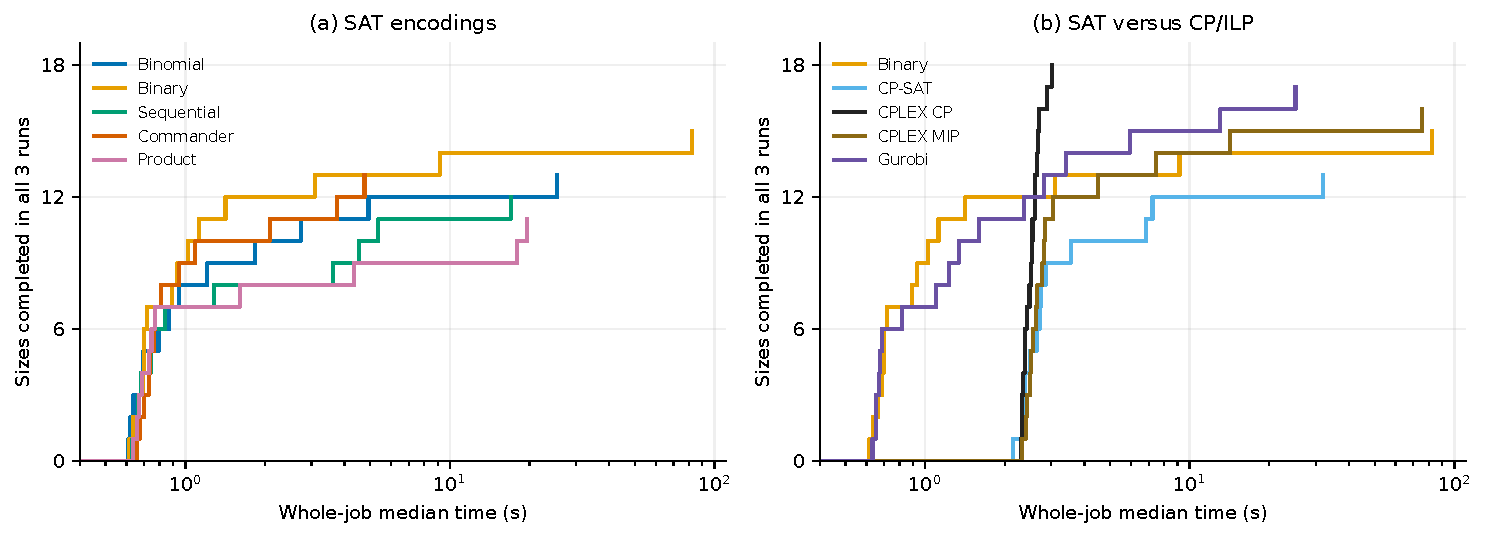
\includegraphics[width=\linewidth]{figures/cactus.pdf}
\caption{Số kích thước hoàn tất đủ 3/3 theo ngưỡng trung vị total. Chỉ các nhóm hoàn tất được tính; đường kết thúc ở số kích thước đã giải, không thay lượt chưa hoàn tất bằng điểm 100 giây.}
\label{fig:cactus}
\end{figure}

\subsection{So sánh số biến và số mệnh đề}
\begin{table}[pos=H]
\centering
\footnotesize
\caption{Số biến CNF đầy đủ của năm mã hóa.}
\label{tab:variables}
\setlength{\tabcolsep}{4pt}
\begin{tabular}{@{}lrrrrr@{}}
\toprule
$N$ & Binomial & Binary & Sequential & Commander & Product \\
\midrule
4 & 16 & 48 & 46 & 36 & 16 \\
8 & 64 & 174 & 262 & 154 & 236 \\
9 & 81 & 229 & 341 & 189 & 289 \\
16 & 256 & 572 & 1\,174 & 744 & 820 \\
25 & 625 & 1\,241 & 2\,965 & 1\,813 & 2\,533 \\
27 & 729 & 1\,405 & 3\,473 & 2\,061 & 2\,937 \\
36 & 1\,296 & 2\,328 & 6\,254 & 3\,876 & 4\,732 \\
49 & 2\,401 & 3\,901 & 11\,701 & 7\,265 & 8\,097 \\
64 & 4\,096 & 6\,136 & 20\,086 & 12\,442 & 12\,476 \\
81 & 6\,561 & 9\,441 & 32\,309 & 19\,449 & 18\,221 \\
100 & 10\,000 & 13\,678 & 49\,390 & 30\,536 & 26\,104 \\
125 & 15\,625 & 20\,353 & 77\,365 & 47\,257 & 37\,749 \\
216 & 46\,656 & 55\,988 & 231\,974 & 140\,030 & 94\,672 \\
343 & 117\,649 & 134\,109 & 586\,177 & 355\,969 & 220\,149 \\
512 & 262\,144 & 287\,730 & 1\,307\,638 & 789\,618 & 459\,472 \\
729 & 531\,441 & 571\,069 & 2\,652\,821 & 1\,595\,061 & 859\,721 \\
1000 & 1\,000\,000 & 1\,055\,888 & 4\,993\,990 & 3\,013\,684 & 1\,514\,732 \\
1331 & 1\,771\,561 & 1\,851\,197 & 8\,849\,809 & 5\,326\,901 & 2\,536\,565 \\
\bottomrule
\end{tabular}
\par\smallskip\begin{minipage}{\linewidth}\footnotesize Commander và Product đều là bản đệ quy. Số đếm theo công thức trước tiền xử lý; TIMEOUT không làm giảm kích thước mô hình đầy đủ. Không bao gồm clause học.\end{minipage}
\end{table}

\begin{table}[pos=H]
\centering
\footnotesize
\caption{Số clause đầu vào của năm mã hóa.}
\label{tab:clauses}
\setlength{\tabcolsep}{4pt}
\begin{tabular}{@{}lrrrrr@{}}
\toprule
$N$ & Binomial & Binary & Sequential & Commander & Product \\
\midrule
4 & 84 & 120 & 104 & 124 & 84 \\
8 & 744 & 728 & 592 & 634 & 652 \\
9 & 1\,074 & 1\,114 & 774 & 822 & 826 \\
16 & 6\,352 & 3\,928 & 2\,720 & 3\,176 & 2\,804 \\
25 & 24\,850 & 11\,806 & 6\,950 & 8\,018 & 7\,638 \\
27 & 31\,410 & 13\,890 & 8\,154 & 9\,294 & 8\,930 \\
36 & 75\,252 & 28\,320 & 14\,760 & 17\,276 & 15\,292 \\
49 & 191\,394 & 54\,866 & 27\,734 & 32\,526 & 27\,742 \\
64 & 428\,864 & 95\,576 & 47\,744 & 55\,990 & 45\,620 \\
81 & 872\,802 & 172\,694 & 76\,950 & 89\,322 & 70\,710 \\
100 & 1\,646\,900 & 269\,024 & 117\,800 & 138\,628 & 106\,292 \\
125 & 3\,224\,250 & 426\,574 & 184\,750 & 216\,062 & 161\,882 \\
216 & 16\,703\,352 & 1\,449\,224 & 555\,120 & 647\,438 & 458\,024 \\
343 & 67\,021\,514 & 4\,060\,266 & 1\,404\,242 & 1\,644\,150 & 1\,121\,094 \\
512 & 223\,173\,120 & 9\,262\,424 & 3\,134\,464 & 3\,662\,390 & 2\,439\,384 \\
729 & 644\,639\,634 & 20\,558\,002 & 6\,361\,254 & 7\,421\,982 & 4\,824\,850 \\
1000 & 1\,664\,669\,000 & 39\,300\,904 & 11\,978\,000 & 13\,999\,546 & 8\,907\,744 \\
1331 & 3\,926\,372\,802 & 75\,151\,050 & 21\,229\,450 & 24\,787\,642 & 15\,533\,774 \\
\bottomrule
\end{tabular}
\par\smallskip\begin{minipage}{\linewidth}\footnotesize Commander và Product đều là bản đệ quy. Số đếm theo công thức trước tiền xử lý; TIMEOUT không làm giảm kích thước mô hình đầy đủ. Không bao gồm clause học.\end{minipage}
\end{table}

\begin{figure}[pos=H]\centering
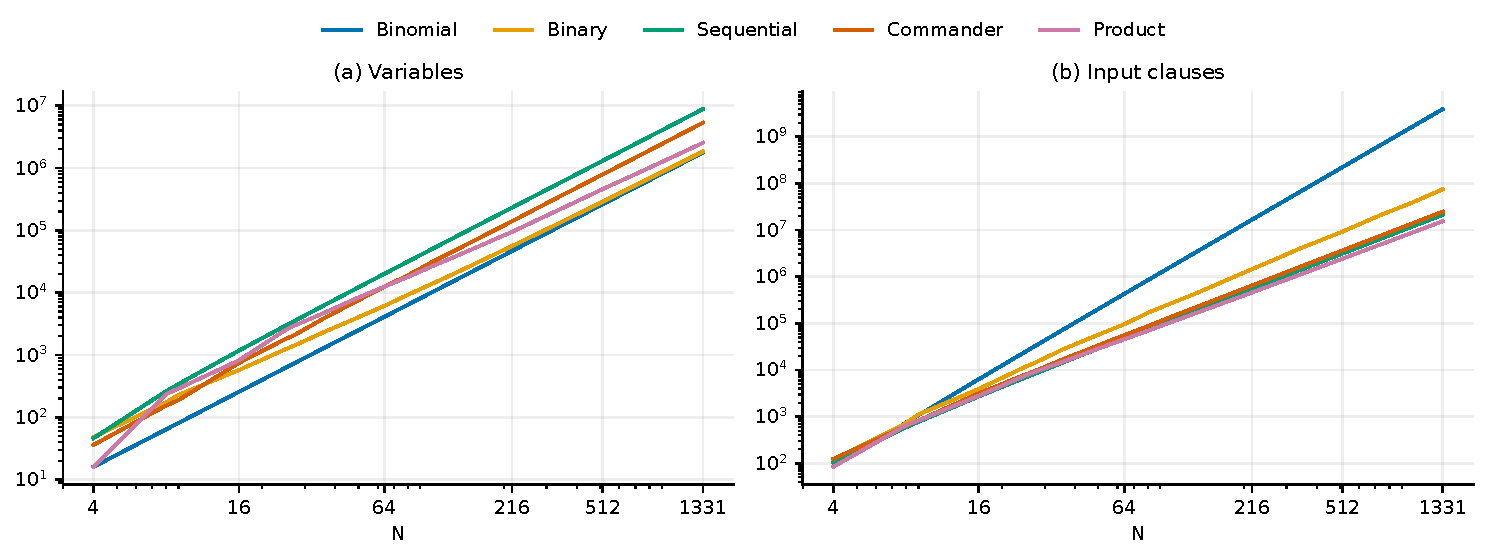
\includegraphics[width=\linewidth]{figures/formula_sizes.pdf}
\caption{Kích thước CNF đầy đủ theo công thức. Hai trục dùng thang log. Commander/Product là bản đệ quy; điểm có số đếm không chứng minh lượt tương ứng đã sinh hoặc nạp hết CNF.}
\label{fig:counts}
\end{figure}
Binomial không thêm biến phụ nên có ít biến nhất, nhưng số clause tăng nhanh nhất. Tại $N=1331$, Binomial có 1\,771\,561 biến và 3\,926\,372\,802 clause. Binary chỉ tăng lên 1\,851\,197 biến, nhưng vẫn có 75\,151\,050 clause. Sequential có 8\,849\,809 biến và 21\,229\,450 clause; Commander có 5\,326\,901 biến và 24\,787\,642 clause; Product có 2\,536\,565 biến và 15\,533\,774 clause.

Như vậy Product có ít clause nhất tại kích thước lớn nhất, còn Sequential dùng nhiều biến nhất trong năm cấu hình. Các con số phù hợp với cấu trúc: Binary chia sẻ một mã bit trong mỗi nhóm, Sequential cần chuỗi gần bằng độ dài nhóm, Commander tạo các tầng đại diện và Product phân rã qua các tập tọa độ. Tuy nhiên, các đặc trưng kích thước chưa đủ dự đoán khả năng hoàn tất trong 100 giây, như các kết quả thời gian sau đây cho thấy.

\subsection{So sánh thời gian giữa các mã hóa SAT}
\begin{table}[pos=H]
\centering
\small
\caption{Thời gian sinh, nạp và giải SAT: $T_{\mathrm{work}}$ (giây).}
\label{tab:sat_work}
\setlength{\tabcolsep}{4pt}
\begin{tabular}{@{}lrrrrr@{}}
\toprule
$N$ & Binomial & Binary & Sequential & Commander & Product \\
\midrule
4 & 0.000295 & 0.000424 & 0.000388 & 0.000500 & 0.000322 \\
8 & 0.001347 & 0.001974 & 0.001213 & 0.001939 & 0.002030 \\
9 & 0.001568 & 0.002136 & 0.001609 & 0.002271 & 0.002592 \\
16 & 0.0306 & 0.0183 & 0.0166 & 0.0779 & 0.0143 \\
25 & 0.0335 & 0.0307 & 0.0528 & 0.0366 & 0.0353 \\
27 & 0.0516 & 0.0275 & 0.1031 & 0.0642 & 0.1004 \\
36 & 0.0953 & 0.0933 & 0.1389 & 0.1180 & 0.0999 \\
49 & 0.2141 & 0.2645 & 0.6036 & 0.1184 & 0.7945 \\
64 & 0.5004 & 0.2273 & 3.902 & 0.3088 & 18.958 \\
81 & 1.091 & 0.3448 & 2.945 & 0.3738 & 3.648 \\
100 & 1.894 & 0.4430 & 4.715 & 1.395 & 17.319 \\
125 & 3.944 & 0.7298 & 16.299 & 3.015 & 1S+2TO \\
216 & 22.912 & 2.296 & TO & 3.940 & TO \\
343 & TO & 8.089 & TO & TO & TO \\
512 & TO & 81.088 & TO & TO & TO \\
729 & TO & TO & TO & TO & TO \\
1000 & TO & TO & TO & TO & TO \\
1331 & TO & TO & TO & TO & TO \\
\bottomrule
\end{tabular}
\par\smallskip\begin{minipage}{\linewidth}\footnotesize Giá trị số: trung vị của ba lượt SAT có nghiệm hợp lệ. TO: ba TIMEOUT; 2TO+1U: hai TIMEOUT và một UNKNOWN; 1S+2TO: một SAT và hai TIMEOUT. Không thay lượt chưa hoàn tất bằng 0 hoặc 100 giây.\end{minipage}
\end{table}

\begin{table}[pos=H]
\centering
\small
\caption{Thời gian toàn lượt SAT: $T_{\mathrm{total}}$ (giây).}
\label{tab:sat_total}
\setlength{\tabcolsep}{4pt}
\begin{tabular}{@{}lrrrrr@{}}
\toprule
$N$ & Binomial & Binary & Sequential & Commander & Product \\
\midrule
4 & 0.6085 & 0.6645 & 0.6297 & 0.7000 & 0.6335 \\
8 & 0.6199 & 0.6987 & 0.6622 & 0.6723 & 0.6663 \\
9 & 0.6376 & 0.6152 & 0.6808 & 0.6593 & 0.6569 \\
16 & 0.7921 & 0.6893 & 0.6653 & 0.7351 & 0.6843 \\
25 & 0.6953 & 0.6344 & 0.7505 & 0.7693 & 0.7283 \\
27 & 0.6795 & 0.6968 & 0.7408 & 0.7276 & 0.7457 \\
36 & 0.9440 & 0.7163 & 0.8390 & 0.7624 & 0.7660 \\
49 & 0.8694 & 0.9330 & 1.282 & 0.8098 & 1.607 \\
64 & 1.212 & 0.8928 & 4.530 & 0.9501 & 19.578 \\
81 & 1.838 & 1.024 & 3.614 & 1.092 & 4.347 \\
100 & 2.731 & 1.123 & 5.370 & 2.084 & 17.965 \\
125 & 4.929 & 1.419 & 16.970 & 3.745 & 1S+2TO \\
216 & 25.469 & 3.085 & TO & 4.760 & TO \\
343 & TO & 9.145 & TO & TO & TO \\
512 & TO & 82.550 & TO & TO & TO \\
729 & TO & TO & TO & TO & TO \\
1000 & TO & TO & TO & TO & TO \\
1331 & TO & TO & TO & TO & TO \\
\bottomrule
\end{tabular}
\par\smallskip\begin{minipage}{\linewidth}\footnotesize Giá trị số: trung vị của ba lượt SAT có nghiệm hợp lệ. TO: ba TIMEOUT; 2TO+1U: hai TIMEOUT và một UNKNOWN; 1S+2TO: một SAT và hai TIMEOUT. Không thay lượt chưa hoàn tất bằng 0 hoặc 100 giây.\end{minipage}
\end{table}

\begin{figure}[pos=H]\centering
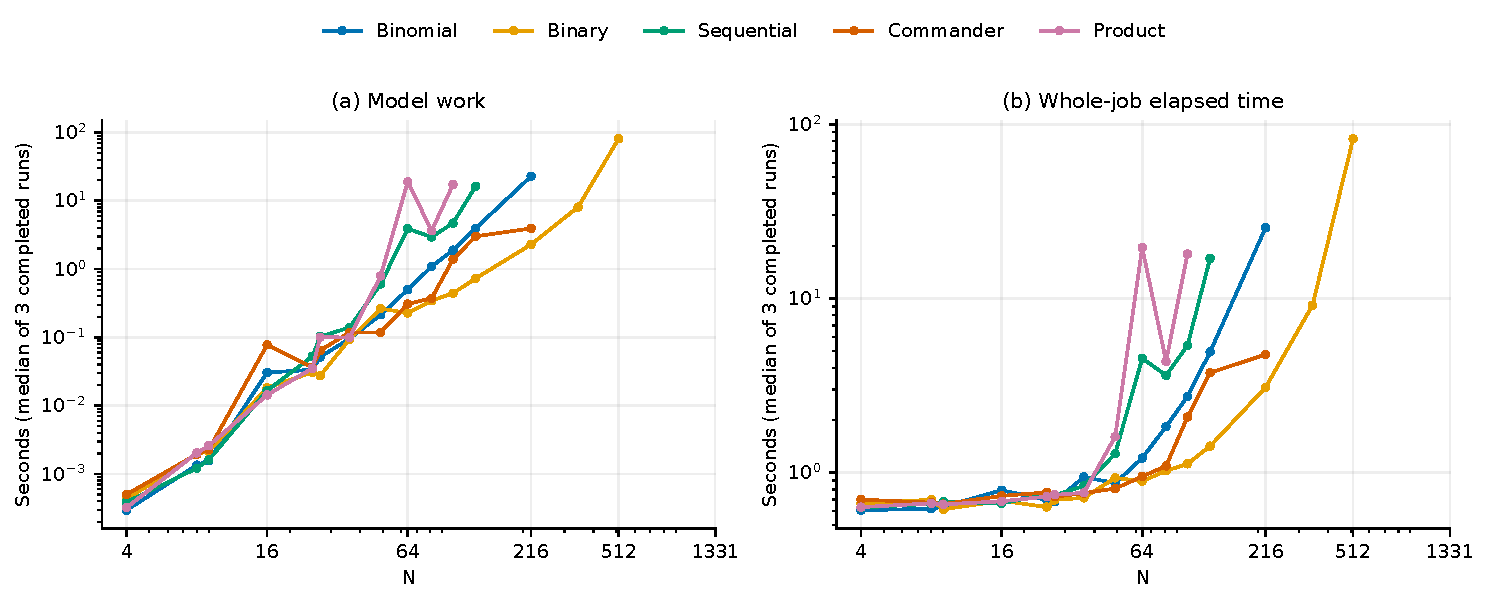
\includegraphics[width=\linewidth]{figures/sat_runtime.pdf}
\caption{Trung vị thời gian SAT: phần xử lý mô hình và giải (trái), toàn lượt (phải). Chỉ vẽ các nhóm hoàn tất 3/3; các trục thời gian dùng thang log.}
\label{fig:sat-time}
\end{figure}
Binary đạt mức độ hoàn tất cao nhất trong các cấu hình SAT: 15/18 kích thước, đến $N=512$. Tại $N=216$, trung vị work của Binary là 2.296 giây, Commander 3.940 giây và Binomial 22.912 giây; Sequential và Product đều timeout. Tại $N=512$, Binary cần 81.088 giây work và 82.550 giây total, còn bốn mã hóa SAT khác đều timeout. Đây là ưu thế của Binary trong bộ cài đặt, backend và tập đầu vào hiện tại, không phải một thứ tự ưu việt cho mọi bài SAT.

Ở kích thước nhỏ, thứ hạng thay đổi: Binomial nhanh nhất theo work tại $N=4,9$, Sequential tại $N=8$ và Product tại $N=16$. Tốc độ cũng không tăng đơn điệu theo $N$: work của Product giảm từ 18.958 giây tại $N=64$ xuống 3.648 giây tại $N=81$, dù công thức lớn hơn. Vì thế không nên suy thời gian ở $N$ tiếp theo chỉ từ đường tăng số clause.

\begin{table}[pos=H]
\centering
\small
\caption{Đối chiếu với Binomial trên tập cả hai hoàn tất 3/3.}
\label{tab:pairwise_binomial}
\setlength{\tabcolsep}{4pt}
\begin{tabular}{@{}lrrrr@{}}
\toprule
Encoding & $|S|$ & Nhanh hơn & Chậm hơn & Hệ số hình học \\
\midrule
Binary & 13 & 9 & 4 & 1.762 \\
Sequential & 12 & 2 & 10 & 0.534 \\
Commander & 13 & 6 & 7 & 1.145 \\
Product & 11 & 1 & 10 & 0.426 \\
\bottomrule
\end{tabular}
\par\smallskip\begin{minipage}{\linewidth}\footnotesize Dùng $T_{work}$. Hệ số lớn hơn 1 nghĩa là nhanh hơn Binomial. Tập so sánh khác nhau giữa các hàng, nên không dùng làm xếp hạng chung.\end{minipage}
\end{table}

Với $S$ là tập kích thước cả một mã hóa $E$ và Binomial đều hoàn tất đủ ba lượt, hệ số đối chiếu được tính bằng
\[
G_E=\exp\left(\frac{1}{|S|}\sum_{N\in S}
\log\frac{\widetilde T_{\mathrm{work}}^{\mathrm{Binomial}}(N)}
{\widetilde T_{\mathrm{work}}^{E}(N)}\right).
\]
Binary nhanh hơn Binomial ở 9/13 kích thước chung, hệ số hình học 1.762. Commander nhanh hơn ở 6/13, hệ số 1.145. Sequential và Product có hệ số lần lượt 0.534 và 0.426 trên các tập chung riêng. Những hệ số này không tính các lượt chưa hoàn tất và tập $S$ khác nhau, nên cần đọc cùng bảng mức độ hoàn tất, không dùng riêng để xếp hạng toàn bộ phương pháp.

\begin{figure}[pos=H]\centering
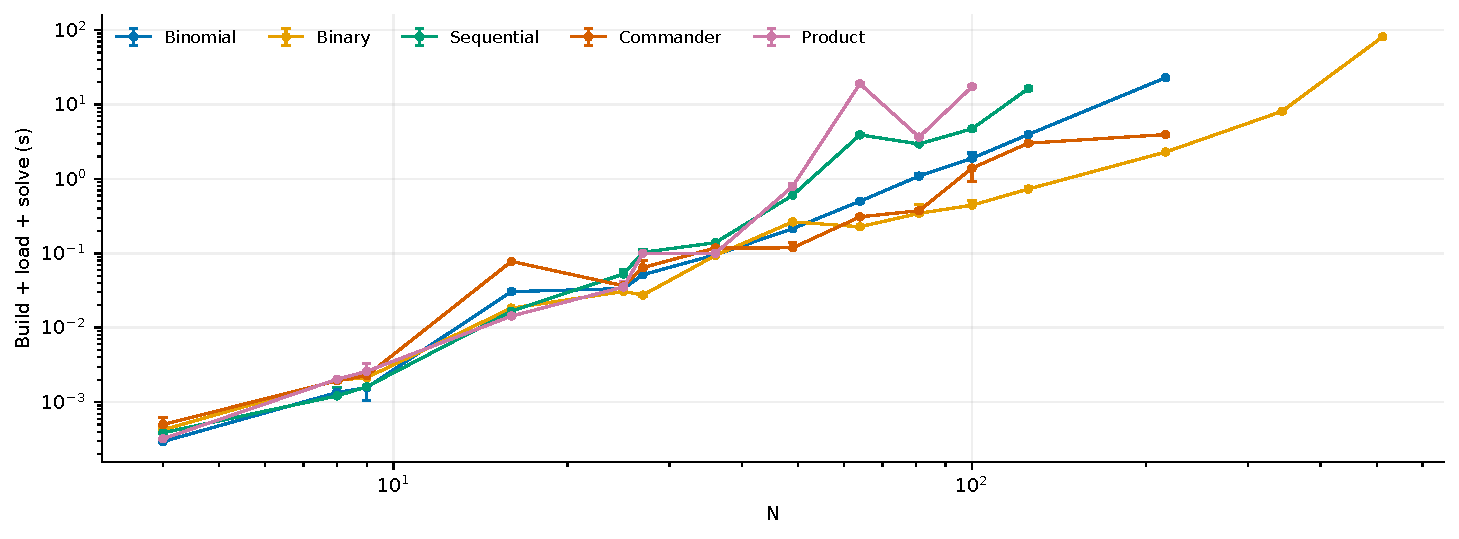
\includegraphics[width=\linewidth]{figures/sat_iqr.pdf}
\caption{Trung vị và khoảng từ Q1 đến Q3 của work trên ba lần lặp hoàn tất. Thanh sai số mô tả độ phân tán, không phải khoảng tin cậy.}
\label{fig:iqr}
\end{figure}
Ví dụ Binary tại $N=81$ có IQR/work trung vị 35.9\%, trong khi tại $N=216$ là 3.0\%. Khác biệt này cho thấy cần giữ các lượt thô thay vì chỉ lưu một thời gian duy nhất. Ba lần lặp chưa đủ để đưa ra kiểm định thống kê mạnh hoặc suy diễn độ ổn định trên nhiều máy.

\subsection{Vì sao ít clause hơn chưa chắc giải nhanh hơn?}
\begin{table}[pos=H]
\centering
\small
\caption{Số clause và công việc tìm kiếm của Glucose3 tại N=64.}
\label{tab:counterexample}
\setlength{\tabcolsep}{4pt}
\begin{tabular}{@{}lrrrr@{}}
\toprule
Mã hóa & Clause & Solve (s) & Xung đột & Lan truyền \\
\midrule
Binomial & 428\,864 & 0.0229 & 317 & 30\,574 \\
Binary & 95\,576 & 0.1026 & 876 & 220\,738 \\
Sequential & 47\,744 & 3.839 & 9\,471 & 3\,899\,877 \\
Commander & 55\,990 & 0.2145 & 1\,231 & 486\,461 \\
Product & 45\,620 & 18.884 & 45\,055 & 12\,682\,652 \\
\bottomrule
\end{tabular}
\par\smallskip\begin{minipage}{\linewidth}\footnotesize Bộ đếm xung đột và lan truyền trùng nhau giữa ba lượt của mỗi mã hóa ở N=64. Thời gian là trung vị; các mã hóa có cấu trúc khác nhau.\end{minipage}
\end{table}

Tại $N=64$, Product chỉ có 45\,620 clause nhưng solve trung vị khoảng 18.884 giây. Binomial có 428\,864 clause, nhiều hơn khoảng 9.4 lần, nhưng solve chỉ khoảng 0.0229 giây. Product ghi nhận 45\,055 xung đột và 12\,682\,652 lần lan truyền, trong khi Binomial lần lượt là 317 và 30\,574. Sequential cũng có ít clause hơn Binary nhưng thời gian solve lớn hơn.

Các số đếm tìm kiếm hỗ trợ nhận xét rằng sự khác biệt không chỉ nằm ở chi phí Python: cấu trúc ràng buộc dẫn tới lượng công việc khác nhau bên trong Glucose3. Chúng chưa chứng minh duy nhất một cơ chế gây chậm, vì thứ tự clause, đánh số biến, quyết định phân nhánh và clause học đều có thể ảnh hưởng. Kết luận phù hợp là kích thước CNF cần được đánh giá cùng hành vi tìm kiếm thực tế.

Tại điểm này, bộ đếm xung đột và lan truyền trùng nhau giữa ba lần lặp của mỗi mã hóa. Do đó không có cơ sở quy mọi dao động thời gian cho sự ngẫu nhiên của SAT solver. Các lượt lặp với cấu hình seed không đổi còn phản ánh biến động của môi trường thực thi.

\subsection{Chi phí khởi động và phân rã thời gian}
\begin{table}[pos=H]
\centering
\small
\caption{Thành phần thời gian SAT tại N=4 (mili giây).}
\label{tab:small_n}
\setlength{\tabcolsep}{4pt}
\begin{tabular}{@{}lrrrrr@{}}
\toprule
Mã hóa & Khởi động & Thiết lập & $T_{work}$ & Solve & $T_{total}$ \\
\midrule
Binomial & 478.149 & 106.422 & 0.295 & 0.061 & 608.488 \\
Binary & 513.512 & 131.196 & 0.424 & 0.085 & 664.473 \\
Sequential & 504.904 & 112.106 & 0.388 & 0.064 & 629.726 \\
Commander & 547.531 & 125.069 & 0.500 & 0.079 & 700.005 \\
Product & 488.594 & 118.623 & 0.322 & 0.063 & 633.508 \\
\bottomrule
\end{tabular}
\par\smallskip\begin{minipage}{\linewidth}\footnotesize Mỗi cột là một trung vị riêng. Trung vị tổng không nhất thiết bằng tổng các trung vị thành phần.\end{minipage}
\end{table}

Ở $N=4$, work của các mã hóa SAT nằm khoảng 0.295--0.500 mili giây, trong khi total khoảng 608--700 mili giây. Phần khởi động và thiết lập chiếm phần lớn khoảng chênh lệch. So total của chương trình có worker riêng với solve của chương trình chạy sẵn trong một tiến trình sẽ tạo khác biệt hàng nghìn lần dù công việc SAT gần tương đương.

\begin{table}[pos=H]
\centering
\small
\caption{Phân rã thời gian tại N=216 (giây).}
\label{tab:phase_216}
\setlength{\tabcolsep}{4pt}
\begin{tabular}{@{}lrrrrr@{}}
\toprule
Phương pháp & Build & Load & Solve & $T_{work}$ & $T_{total}$ \\
\midrule
Binomial & 5.943 & 15.416 & 1.237 & 22.912 & 25.469 \\
Binary & 0.5317 & 1.298 & 0.4549 & 2.296 & 3.085 \\
Sequential & TO & TO & TO & TO & TO \\
Commander & 0.3939 & 0.7232 & 2.818 & 3.940 & 4.760 \\
Product & TO & TO & TO & TO & TO \\
CP-SAT & 0.006869 & -- & 29.904 & 29.911 & 32.014 \\
CPLEX CP & 0.003330 & -- & 0.0830 & 0.0863 & 2.422 \\
CPLEX MIP & 0.6064 & -- & 1.150 & 1.768 & 4.501 \\
Gurobi & 0.7344 & -- & 1.936 & 2.673 & 3.397 \\
\bottomrule
\end{tabular}
\par\smallskip\begin{minipage}{\linewidth}\footnotesize Mỗi cột là một trung vị riêng; tổng các trung vị pha có thể khác trung vị work. Load chỉ áp dụng cho SAT; dấu -- của native không phải một pha nạp được đo bằng 0.\end{minipage}
\end{table}

Tại $N=216$, Binomial có trung vị build 5.943 giây và load 15.416 giây, lớn hơn rõ rệt solve 1.237 giây. Binary giảm phần build/load xuống 0.532 và 1.298 giây; Commander có build/load thấp hơn nữa nhưng solve 2.818 giây, lớn hơn Binary 0.455 giây. Các trung vị pha không bắt buộc cộng lại bằng trung vị work, vì chúng có thể đến từ các lượt khác nhau.

\begin{figure}[pos=H]\centering
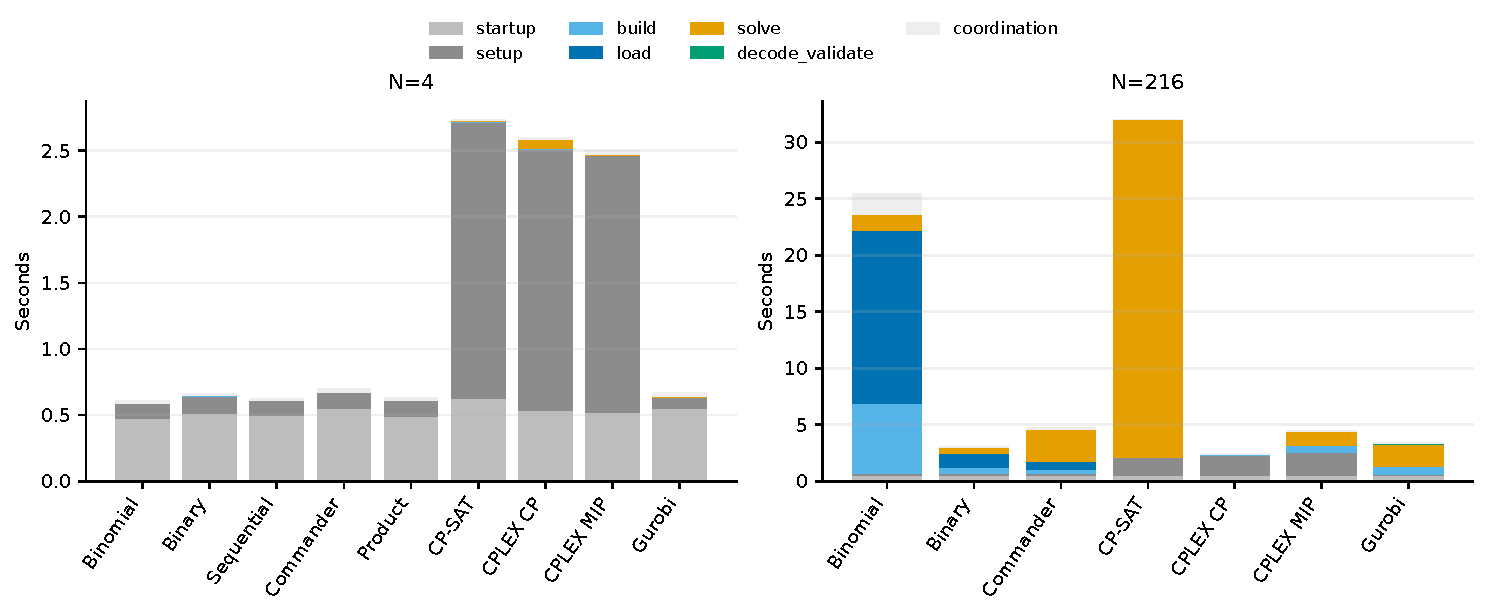
\includegraphics[width=\linewidth]{figures/phase_breakdown.pdf}
\caption{Phân rã một lượt thực tại $N=4$ và $N=216$. Với mỗi cấu hình, chọn lượt có total ở vị trí trung vị; các cột chồng vì vậy thuộc cùng một lượt. Coordination là phần total còn lại sau các pha được ghi.}
\label{fig:phases}
\end{figure}

\subsection{Đối sánh SAT với CP-SAT, CPLEX CP, CPLEX MIP và Gurobi}
\begin{table}[pos=H]
\centering
\small
\caption{Thời gian xây mô hình và gọi giải CP/ILP: $T_{\mathrm{work}}$ (giây).}
\label{tab:native_work}
\setlength{\tabcolsep}{4pt}
\begin{tabular}{@{}lrrrr@{}}
\toprule
$N$ & CP-SAT & CPLEX CP & CPLEX MIP & Gurobi \\
\midrule
4 & 0.0142 & 0.0694 & 0.0146 & 0.0106 \\
8 & 0.0217 & 0.0642 & 0.0125 & 0.009471 \\
9 & 0.0237 & 0.0617 & 0.0138 & 0.009109 \\
16 & 0.0459 & 0.0569 & 0.0214 & 0.0393 \\
25 & 0.0962 & 0.0655 & 0.0340 & 0.0202 \\
27 & 0.1112 & 0.0609 & 0.0350 & 0.0201 \\
36 & 0.2155 & 0.0621 & 0.0528 & 0.0311 \\
49 & 0.4258 & 0.0619 & 0.0833 & 0.1921 \\
64 & 0.7318 & 0.0714 & 0.1399 & 0.0758 \\
81 & 1.395 & 0.0738 & 0.1896 & 0.3590 \\
100 & 3.372 & 0.0727 & 0.2943 & 0.4322 \\
125 & 4.959 & 0.0734 & 0.4708 & 1.187 \\
216 & 29.911 & 0.0863 & 1.768 & 2.673 \\
343 & 2TO+1U & 0.1040 & 4.965 & 1.969 \\
512 & TO & 0.1832 & 10.909 & 4.719 \\
729 & 2TO+1U & 0.2148 & TO & 10.777 \\
1000 & TO & 0.4710 & 72.076 & 21.868 \\
1331 & TO & 0.5211 & TO & TO \\
\bottomrule
\end{tabular}
\par\smallskip\begin{minipage}{\linewidth}\footnotesize Giá trị số: trung vị của ba lượt SAT có nghiệm hợp lệ. TO: ba TIMEOUT; 2TO+1U: hai TIMEOUT và một UNKNOWN; 1S+2TO: một SAT và hai TIMEOUT. Không thay lượt chưa hoàn tất bằng 0 hoặc 100 giây.\end{minipage}
\end{table}

\begin{table}[pos=H]
\centering
\small
\caption{Thời gian toàn lượt CP/ILP (giây).}
\label{tab:native_total}
\setlength{\tabcolsep}{4pt}
\begin{tabular}{@{}lrrrr@{}}
\toprule
$N$ & CP-SAT & CPLEX CP & CPLEX MIP & Gurobi \\
\midrule
4 & 2.735 & 2.598 & 2.499 & 0.6738 \\
8 & 2.338 & 2.545 & 2.324 & 0.6705 \\
9 & 2.486 & 2.352 & 2.775 & 0.6508 \\
16 & 2.145 & 2.295 & 2.626 & 0.8176 \\
25 & 2.358 & 2.522 & 2.505 & 0.6522 \\
27 & 2.382 & 2.480 & 2.397 & 0.6327 \\
36 & 2.638 & 2.376 & 2.832 & 0.6870 \\
49 & 2.713 & 2.314 & 2.423 & 1.338 \\
64 & 2.851 & 2.319 & 2.652 & 1.231 \\
81 & 3.547 & 2.697 & 2.555 & 1.597 \\
100 & 6.843 & 2.653 & 2.812 & 1.099 \\
125 & 7.232 & 2.380 & 3.042 & 2.363 \\
216 & 32.014 & 2.422 & 4.501 & 3.397 \\
343 & 2TO+1U & 2.526 & 7.466 & 2.814 \\
512 & TO & 2.597 & 14.195 & 5.927 \\
729 & 2TO+1U & 2.665 & TO & 13.066 \\
1000 & TO & 2.888 & 75.464 & 25.111 \\
1331 & TO & 3.010 & TO & TO \\
\bottomrule
\end{tabular}
\par\smallskip\begin{minipage}{\linewidth}\footnotesize Giá trị số: trung vị của ba lượt SAT có nghiệm hợp lệ. TO: ba TIMEOUT; 2TO+1U: hai TIMEOUT và một UNKNOWN; 1S+2TO: một SAT và hai TIMEOUT. Không thay lượt chưa hoàn tất bằng 0 hoặc 100 giây.\end{minipage}
\end{table}

\begin{figure}[pos=H]\centering
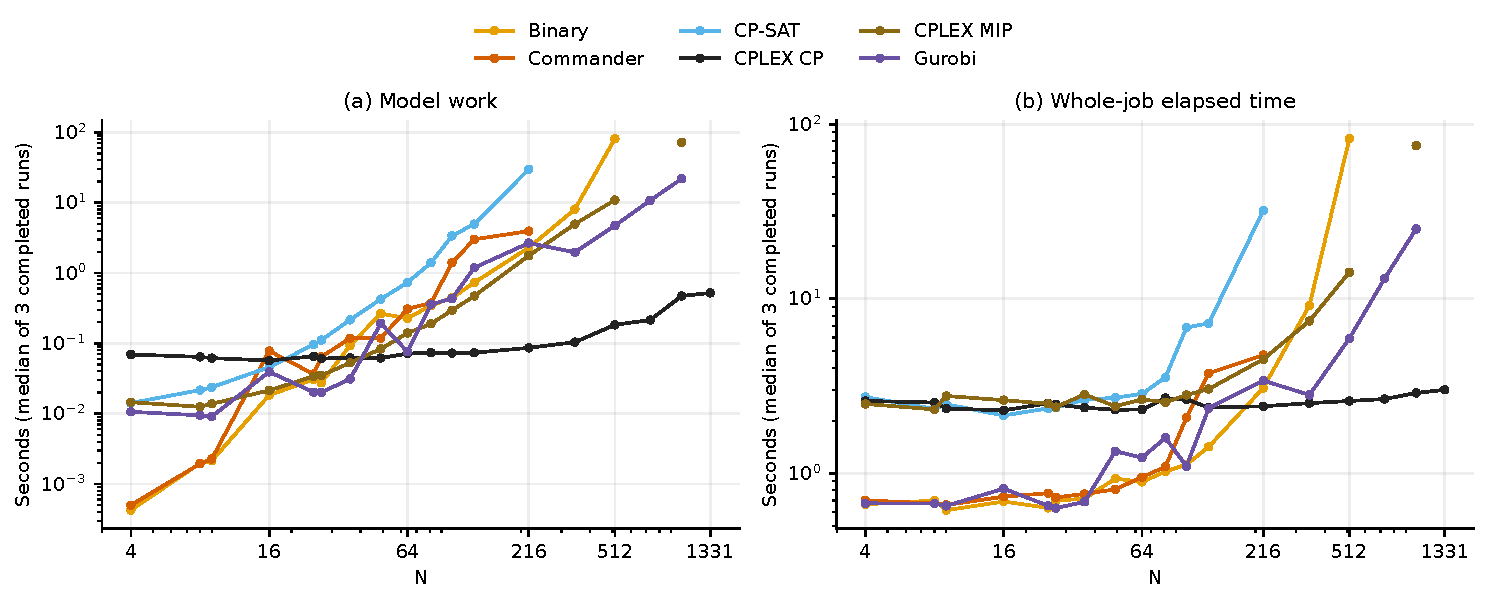
\includegraphics[width=\linewidth]{figures/native_runtime.pdf}
\caption{Binary, Commander và bốn phương pháp đối sánh. Hình tách work với total; chỉ gồm nhóm hoàn tất 3/3.}
\label{fig:native-time}
\end{figure}
CPLEX CP đạt độ bao phủ lớn nhất và có work thấp ở các kích thước lớn: 0.0863 giây tại $N=216$, 0.1832 giây tại $N=512$ và 0.5211 giây tại $N=1331$. Total tương ứng khoảng 2.422, 2.597 và 3.010 giây. Sự chênh lệch work--total phản ánh phần thiết lập còn đáng kể ngay cả khi lời gọi CP hoàn thành nhanh.

Ở $N=512$, Binary cần 81.088 giây work, CPLEX MIP 10.909 giây và Gurobi 4.719 giây. Tại $N=1000$, CPLEX MIP hoàn tất với work 72.076 giây và Gurobi với 21.868 giây, trong khi mọi SAT encoding đều timeout. CPLEX MIP timeout ở $N=729$ nhưng hoàn tất ở $N=1000$; điều này tiếp tục cho thấy độ khó tìm kiếm không đơn điệu theo kích thước. CP-SAT hoàn tất đến $N=216$, rồi các kích thước lớn hơn kết thúc bằng TIMEOUT hoặc UNKNOWN.

\begin{table}[pos=H]
\centering
\small
\caption{Số kích thước có trung vị nhanh nhất trên tập chung.}
\label{tab:matched_winners}
\setlength{\tabcolsep}{4pt}
\begin{tabular}{@{}lrr@{}}
\toprule
Phương pháp & Theo $T_{work}$ & Theo $T_{total}$ \\
\midrule
Binomial & 2 & 2 \\
Binary & 0 & 4 \\
Sequential & 1 & 1 \\
Commander & 0 & 1 \\
Product & 1 & 0 \\
CP-SAT & 0 & 0 \\
CPLEX CP & 4 & 0 \\
CPLEX MIP & 0 & 0 \\
Gurobi & 3 & 3 \\
\bottomrule
\end{tabular}
\par\smallskip\begin{minipage}{\linewidth}\footnotesize Tập chung gồm 11 kích thước: 4, 8, 9, 16, 25, 27, 36, 49, 64, 81, 100. Mỗi kích thước có trọng số bằng nhau; không thay thế đánh giá mức độ hoàn tất.\end{minipage}
\end{table}

Tập mà cả chín cấu hình đều hoàn tất gồm 11 kích thước từ 4 đến 100 trong $\mathcal N$. Theo work, CPLEX CP nhanh nhất ở bốn kích thước, Gurobi ở ba, Binomial ở hai, Sequential và Product mỗi phương pháp ở một. Theo total, Binary dẫn đầu ở bốn kích thước còn CPLEX CP không dẫn đầu ở kích thước nào trong tập chung này. Hai cách đo trả lời hai câu hỏi khác nhau: tốc độ xử lý mô hình và giải sau thiết lập, hoặc độ trễ thực thi toàn lượt.

\begin{table}[pos=H]
\centering
\small
\caption{Kích thước mô hình CP và MIP ở giao diện người dùng.}
\label{tab:native_size}
\setlength{\tabcolsep}{4pt}
\begin{tabular}{@{}lrrrr@{}}
\toprule
$N$ & Biến CP & AllDifferent & Biến MIP & Ràng buộc MIP \\
\midrule
4 & 4 & 3 & 16 & 22 \\
216 & 216 & 3 & 46\,656 & 1\,294 \\
1331 & 1331 & 3 & 1\,771\,561 & 7\,984 \\
\bottomrule
\end{tabular}
\par\smallskip\begin{minipage}{\linewidth}\footnotesize Không quy đổi biến nguyên hoặc ràng buộc mức cao thành biến/clause CNF. Không phải số lượng bên trong solver sau presolve.\end{minipage}
\end{table}

Ba AllDifferent có thể biểu diễn các quan hệ rộng trên miền của $N$ biến nguyên, trong khi mô hình ô cờ SAT/MIP sử dụng $N^2$ biến Boolean/nhị phân. Đây là khác biệt về cách biểu diễn mà backend nhận được, không phải bằng chứng rằng ba ràng buộc CP chỉ có chi phí bằng ba clause. Thực nghiệm so sánh cả mô hình lẫn bộ giải; không cô lập riêng chất lượng thuật toán nội bộ của các engine.

\subsection{RSS và tài nguyên bộ nhớ}
\begin{table}[pos=H]
\centering
\small
\caption{Trung vị đỉnh RSS quan sát (SAT, MiB).}
\label{tab:sat_ram}
\setlength{\tabcolsep}{4pt}
\begin{tabular}{@{}lrrrrr@{}}
\toprule
$N$ & Binomial & Binary & Sequential & Commander & Product \\
\midrule
4 & 27.8 & 27.8 & 27.8 & 27.8 & 27.9 \\
8 & 27.6 & 27.8 & 27.8 & 27.7 & 27.9 \\
9 & 28.1 & 28.2 & 27.9 & 28.0 & 27.8 \\
16 & 29.2 & 28.5 & 28.2 & 28.9 & 28.2 \\
25 & 29.4 & 28.4 & 29.8 & 29.8 & 29.6 \\
27 & 31.2 & 28.7 & 30.0 & 29.9 & 30.1 \\
36 & 33.2 & 30.4 & 31.6 & 31.3 & 30.6 \\
49 & 39.8 & 34.2 & 34.5 & 32.6 & 36.8 \\
64 & 52.4 & 36.0 & 44.5 & 36.8 & 61.2 \\
81 & 71.9 & 40.7 & 45.8 & 39.9 & 49.2 \\
100 & 119.9 & 46.0 & 52.3 & 47.9 & 67.1 \\
125 & 184.2 & 55.6 & 74.0 & 59.5 & 154.8$^{\dagger}$ \\
216 & 1120.7 & 105.4 & 325.0$^{\dagger}$ & 104.2 & 206.9$^{\dagger}$ \\
343 & 3032.1$^{\dagger}$ & 253.1 & 343.5$^{\dagger}$ & 376.5$^{\dagger}$ & 309.2$^{\dagger}$ \\
512 & 3218.7$^{\dagger}$ & 840.9 & 638.4$^{\dagger}$ & 651.8$^{\dagger}$ & 416.6$^{\dagger}$ \\
729 & 3276.9$^{\dagger}$ & 1726.0$^{\dagger}$ & 941.4$^{\dagger}$ & 1116.3$^{\dagger}$ & 685.0$^{\dagger}$ \\
1000 & 3423.3$^{\dagger}$ & 2981.7$^{\dagger}$ & 1590.7$^{\dagger}$ & 1666.2$^{\dagger}$ & 1106.1$^{\dagger}$ \\
1331 & 3162.5$^{\dagger}$ & 3185.7$^{\dagger}$ & 2658.9$^{\dagger}$ & 2578.8$^{\dagger}$ & 1634.2$^{\dagger}$ \\
\bottomrule
\end{tabular}
\par\smallskip\begin{minipage}{\linewidth}\footnotesize $\dagger$: không hoàn tất đủ ba lượt; đây là bộ nhớ đã quan sát trong các lượt chạy, không phải mức RAM cần để giải thành công.\end{minipage}
\end{table}

\begin{table}[pos=H]
\centering
\small
\caption{Trung vị đỉnh RSS quan sát (CP/ILP, MiB).}
\label{tab:native_ram}
\setlength{\tabcolsep}{4pt}
\begin{tabular}{@{}lrrrr@{}}
\toprule
$N$ & CP-SAT & CPLEX CP & CPLEX MIP & Gurobi \\
\midrule
4 & 86.6 & 92.4 & 86.5 & 30.6 \\
8 & 86.8 & 91.6 & 86.5 & 30.8 \\
9 & 86.8 & 86.5 & 86.5 & 30.7 \\
16 & 87.1 & 91.1 & 86.7 & 33.4 \\
25 & 88.0 & 91.2 & 88.0 & 31.2 \\
27 & 88.2 & 93.5 & 88.3 & 31.6 \\
36 & 88.5 & 88.0 & 88.3 & 32.0 \\
49 & 90.6 & 85.7 & 92.0 & 41.5 \\
64 & 94.2 & 91.5 & 94.1 & 36.0 \\
81 & 99.6 & 91.1 & 98.2 & 46.3 \\
100 & 105.7 & 92.4 & 105.3 & 48.7 \\
125 & 118.7 & 92.2 & 114.9 & 66.8 \\
216 & 206.5 & 92.4 & 170.5 & 115.9 \\
343 & 114.9$^{\dagger}$ & 95.9 & 295.0 & 116.7 \\
512 & 111.6$^{\dagger}$ & 102.0 & 523.8 & 221.5 \\
729 & 119.0$^{\dagger}$ & 106.9 & 1035.5$^{\dagger}$ & 426.9 \\
1000 & 156.1$^{\dagger}$ & 127.7 & 1734.2 & 798.1 \\
1331 & 237.2$^{\dagger}$ & 134.3 & 2933.6$^{\dagger}$ & 2943.5$^{\dagger}$ \\
\bottomrule
\end{tabular}
\par\smallskip\begin{minipage}{\linewidth}\footnotesize $\dagger$: không hoàn tất đủ ba lượt; đây là bộ nhớ đã quan sát trong các lượt chạy, không phải mức RAM cần để giải thành công.\end{minipage}
\end{table}

\begin{figure}[pos=H]\centering
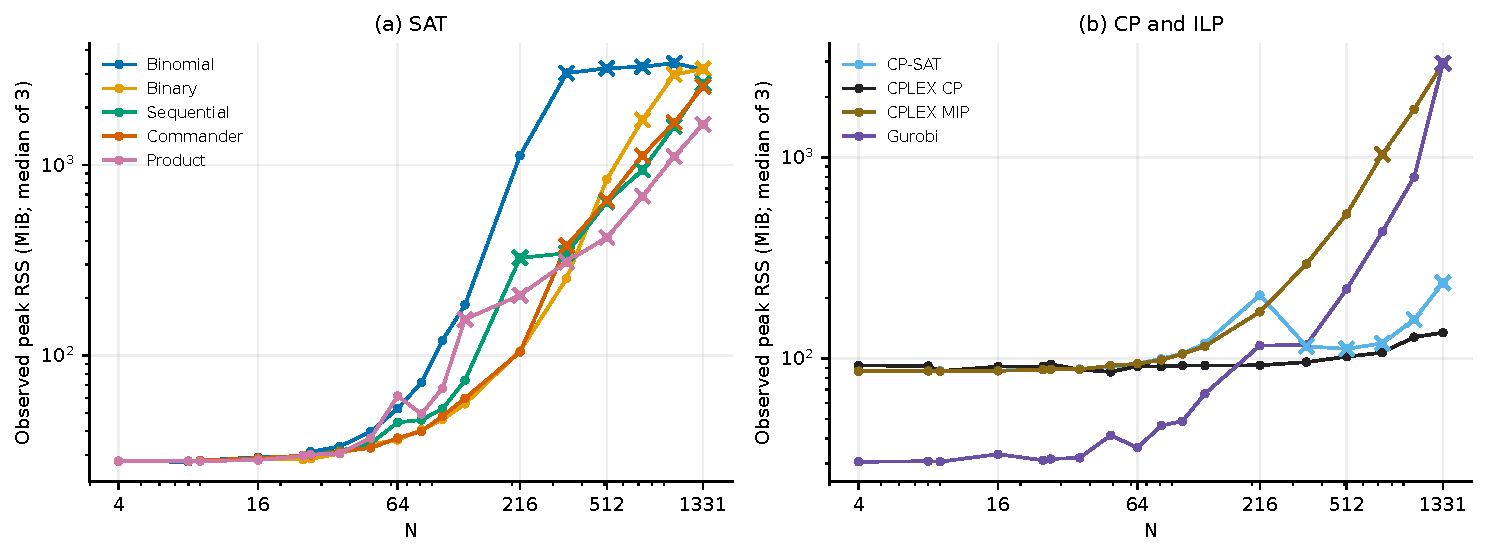
\includegraphics[width=\linewidth]{figures/memory.pdf}
\caption{Trung vị đỉnh RSS quan sát qua ba lượt, kể cả lượt chưa hoàn tất. Dấu x đánh dấu nhóm không hoàn tất đủ 3/3. Hai trục dùng thang log; các điểm bị ngắt không biểu diễn lượng RAM cần để giải thành công.}
\label{fig:memory}
\end{figure}
Tại $N=216$, Binomial dùng RSS đỉnh trung vị khoảng 1120.7 MiB; Binary 105.4 MiB và Commander 104.2 MiB. Ở đây CNF lớn của Binomial đi cùng chi phí nạp và bộ nhớ cao. Tuy nhiên, tại $N=64$, Product có ít clause nhất nhưng RSS 61.2 MiB, cao hơn Binary 36.0 MiB: bộ nhớ còn chứa trạng thái tìm kiếm và clause học, không chỉ công thức đầu vào.

Tại $N=1331$, CPLEX CP hoàn tất với RSS trung vị khoảng 134.3 MiB; Product bị timeout với RSS quan sát trung vị 1634.2 MiB. Hai con số không phải so sánh bộ nhớ để cùng hoàn thành bài toán. Giá trị RSS lớn nhất trong cả 486 lượt là 4631.2 MiB, vẫn dưới ngưỡng cấu hình 6144 MiB; bộ dữ liệu không có MEM\_LIMIT. Điều này chỉ mô tả những gì đã quan sát trước khi các lượt dừng, không chứng minh mọi phương pháp sẽ đủ RAM nếu bỏ giới hạn thời gian.

\subsection{Các lượt bị giới hạn và trường hợp thành công một phần}
\begin{table}[pos=H]
\centering
\footnotesize
\caption{Ba lượt Product đệ quy tại N=125.}
\label{tab:partial_product}
\setlength{\tabcolsep}{4pt}
\begin{tabular}{@{}lrrrrrr@{}}
\toprule
Lượt & Trạng thái & Build (s) & Load (s) & Solve (s) & Total (s) & RSS (MiB) \\
\midrule
1 & SAT & 0.0864 & 0.1827 & 91.748 & 92.942 & 185.1 \\
2 & TIMEOUT & 0.0742 & 0.1598 & -- & 100.027 & 138.4 \\
3 & TIMEOUT & 0.0754 & 0.1525 & -- & 100.019 & 154.8 \\
\bottomrule
\end{tabular}
\par\smallskip\begin{minipage}{\linewidth}\footnotesize Cả ba lượt đã nạp đủ 161.882 clause. Build/load của lượt TIMEOUT là số ghi nhận gần nhất; solve chưa hoàn tất nên không dùng giá trị 0 trong log. Không công bố trung vị hoàn tất của cả cấu hình từ một lượt SAT.\end{minipage}
\end{table}

Product tại $N=125$ là trường hợp duy nhất chỉ thành công một phần: lượt 1 có total 92.942 giây, lượt 2 và 3 timeout xấp xỉ 100 giây. Cả ba đã nạp đủ 161\,882 clause. Vì hai thời gian hoàn tất chưa quan sát được, 92.942 giây không được dùng làm trung vị thời gian hoàn tất của cấu hình. Bảng chính ghi 1S+2TO và bảng chi tiết giữ từng lượt.

\begin{table}[pos=H]
\centering
\small
\caption{Tiến độ nạp CNF trong các lượt SAT bị TIMEOUT.}
\label{tab:timeout_progress}
\setlength{\tabcolsep}{4pt}
\begin{tabular}{@{}lrrr@{}}
\toprule
Encoding & Số TO & Đã báo nạp đủ & Chưa báo nạp đủ \\
\midrule
Binomial & 15 & 3 & 12 \\
Binary & 9 & 6 & 3 \\
Sequential & 18 & 18 & 0 \\
Commander & 15 & 15 & 0 \\
Product & 20 & 20 & 0 \\
\bottomrule
\end{tabular}
\par\smallskip\begin{minipage}{\linewidth}\footnotesize Tiến độ là thông báo gần nhất. Đã nạp đủ không có nghĩa đã giải xong; nhãn phase có thể cũ. Không lấy solve\_s=0 của lượt bị ngắt làm thời gian tìm kiếm.\end{minipage}
\end{table}

Trong 77 lượt TIMEOUT của các phương pháp SAT, 62 lượt đã báo nạp đủ CNF và 15 lượt chưa báo nạp đủ. Các lượt Sequential, Commander và Product bị timeout đều thuộc nhóm đã nạp đủ. Vì thông báo pha có thể chậm hơn tiến trình thực, báo cáo dùng bộ đếm clause để phân biệt tiến độ, không chỉ dựa vào nhãn \texttt{phase}.

\begin{table}[pos=H]
\centering
\footnotesize
\caption{Kích thước đầy đủ và tiến độ nạp tại N=1331.}
\label{tab:progress_1331}
\setlength{\tabcolsep}{4pt}
\begin{tabular}{@{}lrrrr@{}}
\toprule
Encoding & Clause đầy đủ & Nạp: nhỏ nhất & Nạp: lớn nhất & Trạng thái \\
\midrule
Binomial & 3\,926\,372\,802 & 71\,680\,000 & 80\,928\,768 & 3TO \\
Binary & 75\,151\,050 & 65\,363\,968 & 65\,978\,368 & 3TO \\
Sequential & 21\,229\,450 & 21\,229\,450 & 21\,229\,450 & 3TO \\
Commander & 24\,787\,642 & 24\,787\,642 & 24\,787\,642 & 3TO \\
Product & 15\,533\,774 & 15\,533\,774 & 15\,533\,774 & 3TO \\
\bottomrule
\end{tabular}
\par\smallskip\begin{minipage}{\linewidth}\footnotesize Các giá trị nạp là bản cập nhật đã nhận trước khi ngắt. Không phải kích thước CNF rút gọn và không bao gồm clause học.\end{minipage}
\end{table}

Tại $N=1331$, Sequential, Commander và Product đều nạp đủ CNF nhưng không trả nghiệm được chấp nhận trước khi lượt bị dừng. Binomial và Binary chưa báo nạp đủ. Do đó không thể diễn giải tất cả TIMEOUT như việc solver đã được dành riêng đủ 100 giây để tìm kiếm. Tăng RAM đơn thuần cũng không trực tiếp giải quyết các trường hợp chạm thời gian khi RSS vẫn dưới ngưỡng.

\subsection{Đối chiếu tài liệu tham khảo và giới hạn của kết luận}
Bảng thời gian SAT được trình bày theo hàng $N$ và cột encoding, tương ứng cách tổ chức Bảng 4.2 trong tài liệu của Trần Ngọc Bách \citep{bach2024}. Tuy nhiên tài liệu đó dùng CPU i7-1165G7 và cài đặt khác; ở đây còn tách work với total và dùng ba lần lặp. Do đó không lấy tỷ số thời gian giữa hai báo cáo để kết luận encoder hiện tại nhanh hoặc chậm hơn do một thay đổi duy nhất. Tương tự, bộ dữ liệu này không phải phép so sánh có kiểm soát giữa bản một tầng và bản đệ quy.

Có bốn giới hạn cần giữ khi diễn giải. Thứ nhất, chỉ có một máy, một SAT backend và 18 bàn cờ trống; kết quả không đại diện cho N-Queens có hậu cố định hoặc các bài toán lực lượng khác. Thứ hai, ba lần lặp cùng cấu hình mô tả biến động thời gian nhưng không đủ suy diễn thống kê mạnh về mọi seed hay mọi môi trường. Thứ ba, giới hạn toàn lượt làm chi phí khởi động, dựng và nạp mô hình ảnh hưởng mức độ hoàn tất. Thứ tư, RSS lấy mẫu và số đếm mô hình có ý nghĩa khác nhau giữa các họ bộ giải.

Manifest có hash mã nguồn nhưng gói kết quả không thay thế snapshot nguồn tương ứng hoặc commit Git. Phiên bản CP Optimizer engine, tên thương mại CPU và trạng thái nguồn điện cần được bổ sung nếu muốn tái lập sát môi trường gốc. Các kết luận trong báo cáo giới hạn ở cài đặt được mô tả và những số đo đã cung cấp.


\subsection{Tái tạo số liệu và truy vết biểu đồ}
\label{sec:reproducibility}
Quy trình hậu xử lý sử dụng một nguồn thống kê chung cho bảng và hình. Trước khi tổng hợp, chương trình đối chiếu từng trường CSV với bản ghi JSONL theo run ID, kiểm tra đủ lưới 486 lượt và kiểm tra nghiệm. Sau đó các lượt được nhóm theo cặp $(N,\text{phương pháp})$; work được cộng trong từng lượt trước khi tính trung vị. Nhóm chưa hoàn tất đủ ba lần không được đưa vào đường thời gian như một điểm hoàn tất; trạng thái của nó được giữ trong bảng và Hình~\ref{fig:status}.

Số liệu dẫn xuất được lưu vào \texttt{summary\_report.csv}. Khi vẽ, chương trình đồng thời xuất chính các điểm đã sử dụng sang CSV tương ứng từng hình. Nhờ đó, một điểm có thể được kiểm tra ngược qua ba mức: CSV của hình, dòng tổng hợp và ba bản ghi gốc. Chẳng hạn Product tại $N=125$ giữ trạng thái 1S+2TO và không có trung vị hoàn tất trong đường thời gian; lượt thành công vẫn được trình bày riêng ở bảng phân tích thành công một phần. Với hình phân rã pha, CSV giữ run ID của lượt có total trung vị, bảo đảm các thành phần của một cột thuộc cùng một lượt thật.

Sau khi tách mã hậu xử lý thành các module, toàn bộ 24 bảng thực nghiệm, bốn CSV tổng hợp và kết quả audit đã được đối chiếu với bản dựng trước và giữ nguyên số liệu. Sáu kiểm thử kiểm tra các rủi ro tổng hợp: cộng pha trước trung vị; giữ nhóm thành công một phần; phát hiện run ID trùng và số đo CSV/JSONL không khớp; đối chiếu điểm hình với thống kê; và kiểm tra tổng các pha của đúng một lượt. Đây là kiểm chứng phần hậu xử lý, không phải kiểm thử thêm các solver. Chi tiết lệnh chạy và vai trò từng hình ở Phụ lục~\ref{app:reproduce}.
